\subsection{Structural and Decomposition Cryptanalysis}

\renewcommand{\TITLE}{\it Structural and Decomposition Cryptanalysis}

\begin{frame}
\CurTitle{}

\Center{
\textcolor{blue}{Distinguishing} structures and \textcolor{red}{recovering} components
}
\end{frame}


\begin{frame}[t]
\CurTitle{}

\only<1>{
    \begin{textblock*}{4cm}(2cm,1.25cm)
    \includegraphics[width=3.5cm]{figures/blackbox.pdf}
    \end{textblock*}
}
\only<2>{
    \begin{textblock*}{4cm}(2cm,2cm)
    \begin{tabu} to 3.5cm { | X[c] | X[c]| }
 \hline
 $x$ & $E(x)$ \\ 
 \hline
 0 & 182 \\
 1 & 210 \\
 2 & 78 \\
 3 & 251 \\
 4 & 97 \\
%  5 & 83 \\
 \hline
 \multicolumn{2}{|c|}{\ldots} \\
 \hline
 252 & 112 \\
 253 & 19 \\
 254 & 224 \\
 255 & 74 \\
 \hline
\end{tabu}
    \end{textblock*}
}
\only<3->{
    \begin{textblock*}{4cm}(2cm,1.75cm)
        \includegraphics[height=5.75cm]{figures/feistel.pdf}
        \\
        \large \hspace*{0.3cm}
        Feistel Networks
    \end{textblock*}
    
}


\only<6>{
    \begin{textblock*}{4cm}(6.2cm,2cm)
    \begin{tabu} to 3.5cm { | X[c] | X[c]| }
 \hline
 $x$ & $E(x)$ \\ 
 \hline
 0 & 182 \\
 1 & 210 \\
 2 & 78 \\
 3 & 251 \\
 4 & 97 \\
%  5 & 83 \\
 \hline
 \multicolumn{2}{|c|}{\ldots} \\
 \hline
 252 & 112 \\
 253 & 19 \\
 254 & 224 \\
 255 & 74 \\
 \hline
\end{tabu}
    \end{textblock*}
}
\only<7->{
    \begin{textblock*}{4cm}(6cm,1.75cm)
    \begin{center}\includegraphics[height=5cm]{figures/apn.pdf}\end{center}
        \large
        \hspace*{1.1cm} 6-bit APN \\
        \hspace*{0.9cm} Permutation
    \end{textblock*}
}
\only<8->{
    \begin{textblock*}{6cm}(5.55cm,1.6cm)
        \begin{tikzpicture}
        \node[opacity=0.2] {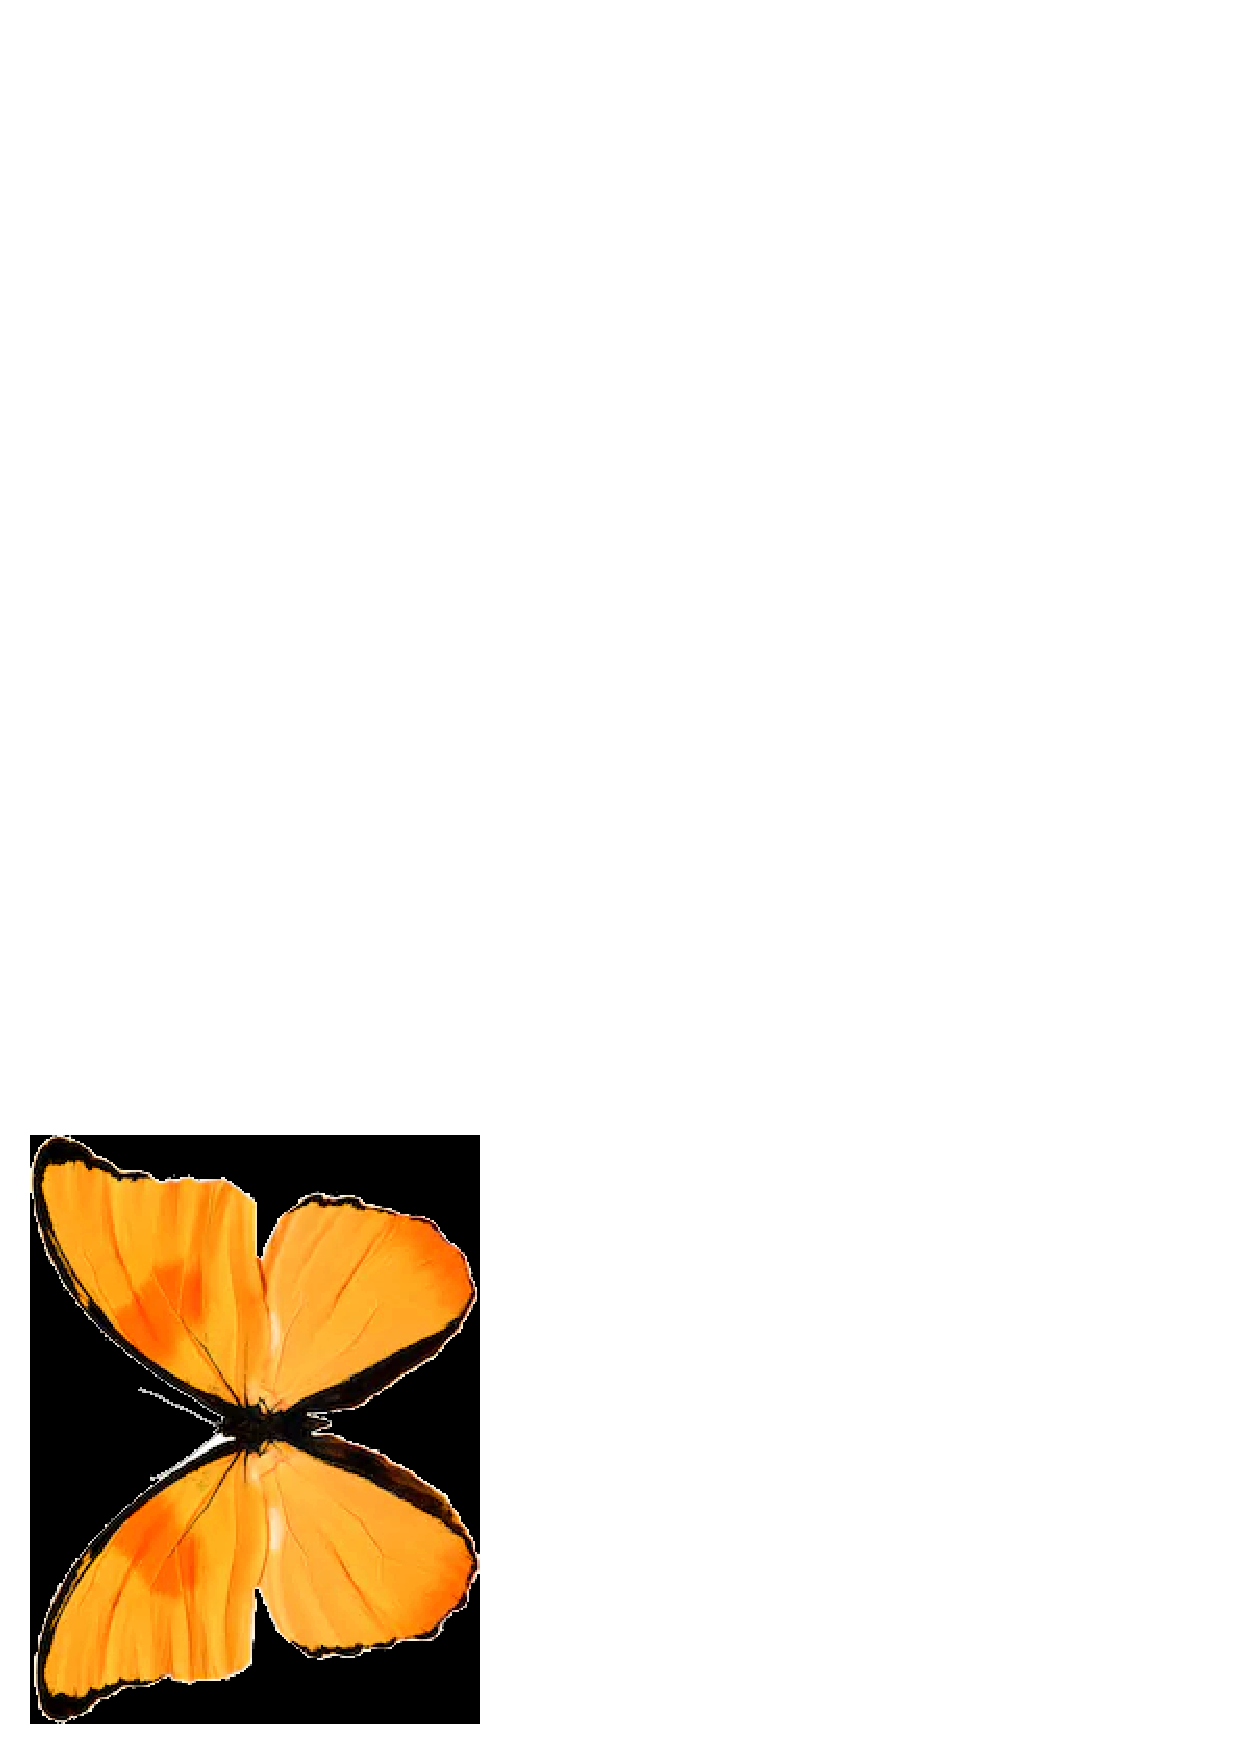
\includegraphics[height=6cm]{figures/butterfly.png}};
        \end{tikzpicture}
    \end{textblock*}
}

\only<4>{
    \begin{textblock*}{4cm}(10cm,2cm)
    \begin{tabu} to 3.5cm { | X[c] | X[c]| }
 \hline
 $x$ & $E(x)$ \\ 
 \hline
 0 & 182 \\
 1 & 210 \\
 2 & 78 \\
 3 & 251 \\
 4 & 97 \\
%  5 & 83 \\
 \hline
 \multicolumn{2}{|c|}{\ldots} \\
 \hline
 252 & 112 \\
 253 & 19 \\
 254 & 224 \\
 255 & 74 \\
 \hline
\end{tabu}
    \end{textblock*}
}
\only<5->{
    \begin{textblock*}{4cm}(10cm,1.75cm)
    \begin{center}\includegraphics[height=5cm]{figures/kuzlog.pdf}\end{center}
        \large \hspace*{0.9cm}
        GOST S-Box
    \end{textblock*}
}

\end{frame}

\begin{frame}
    \CurTitle{}
    
    \nociteparti{mybibFeistel}
    \nociteparti{mybibAPN}
    \nociteparti{mybibKuz1}
    \nociteparti{mybibKuz2}
    \bibliographystyleparti{unsrt}
    \bibliographyparti{mybiblio.bib}
\end{frame}